\documentclass{beamer}
\usepackage{graphicx}
\usepackage{hyperref}
\title{CPP Community Garden Meeting Note}
\author{An Pham}
\institute{Calpoly Pomona}
\date{\today}
\usetheme{Boadilla}
%\usetheme{Berkeley}
\usepackage{graphicx}
\usepackage{booktabs}
\usepackage{hyperref}
\usepackage[english]{babel}

\begin{document}
\frame{\titlepage}

\begin{frame}
\frametitle{Overview}
\begin{enumerate}
  \item Revisit the new sensor kit.
   \item Analysize LORAWAN compared to ECOWITT set up.
   \item Trade study for irrigration system.
   \item Continue work needed.
\end{enumerate}
\end{frame}

\begin{frame}
  \frametitle{Ecowitt Sensors Kit}
  \begin{itemize}
        \item Objectives: Build Remote sensing and Remote Imaging Solution
    \item Success Criteria:
      \begin{itemize}
        \item Easy to deploy / Cost effective.
        \item Set up one time and let it be.
	\item Wifi compatibility.
          \begin{itemize}
            \item Mounting on rooftop.
            \item Mounting on tree.
          \end{itemize}
      \end{itemize}
    \item Limitation: 
      \begin{itemize}
        \item Require 2.4gz bandwidth (set up router to run in this mode).
	\item Wifi Rounter is required.
      \end{itemize}
  \end{itemize}
 \end{frame}

\begin{frame}
  \frametitle{Ecowitt Sensors Kit Cont.}
  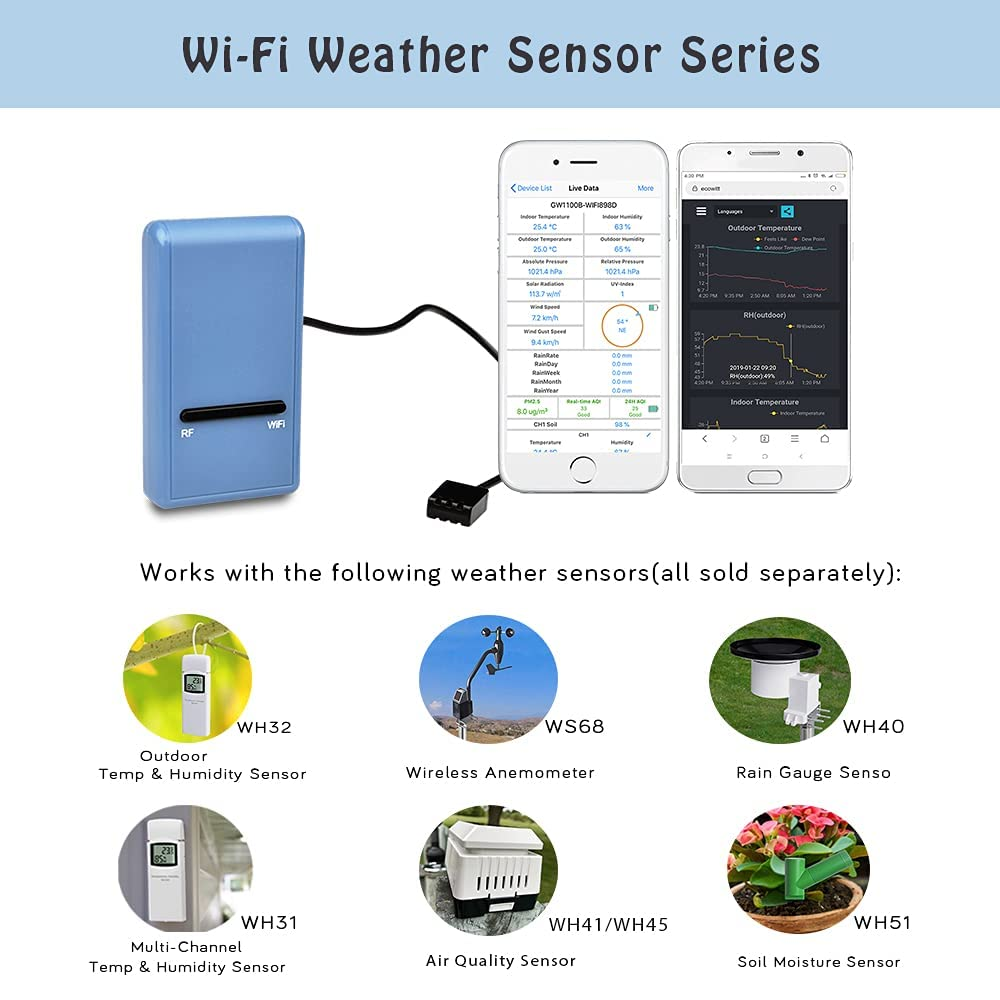
\includegraphics[scale=0.2]{sensors-collection.jpg}
\end{frame}

\begin{frame}
  \frametitle{Ecowitt Sensors Kit Cont.}
  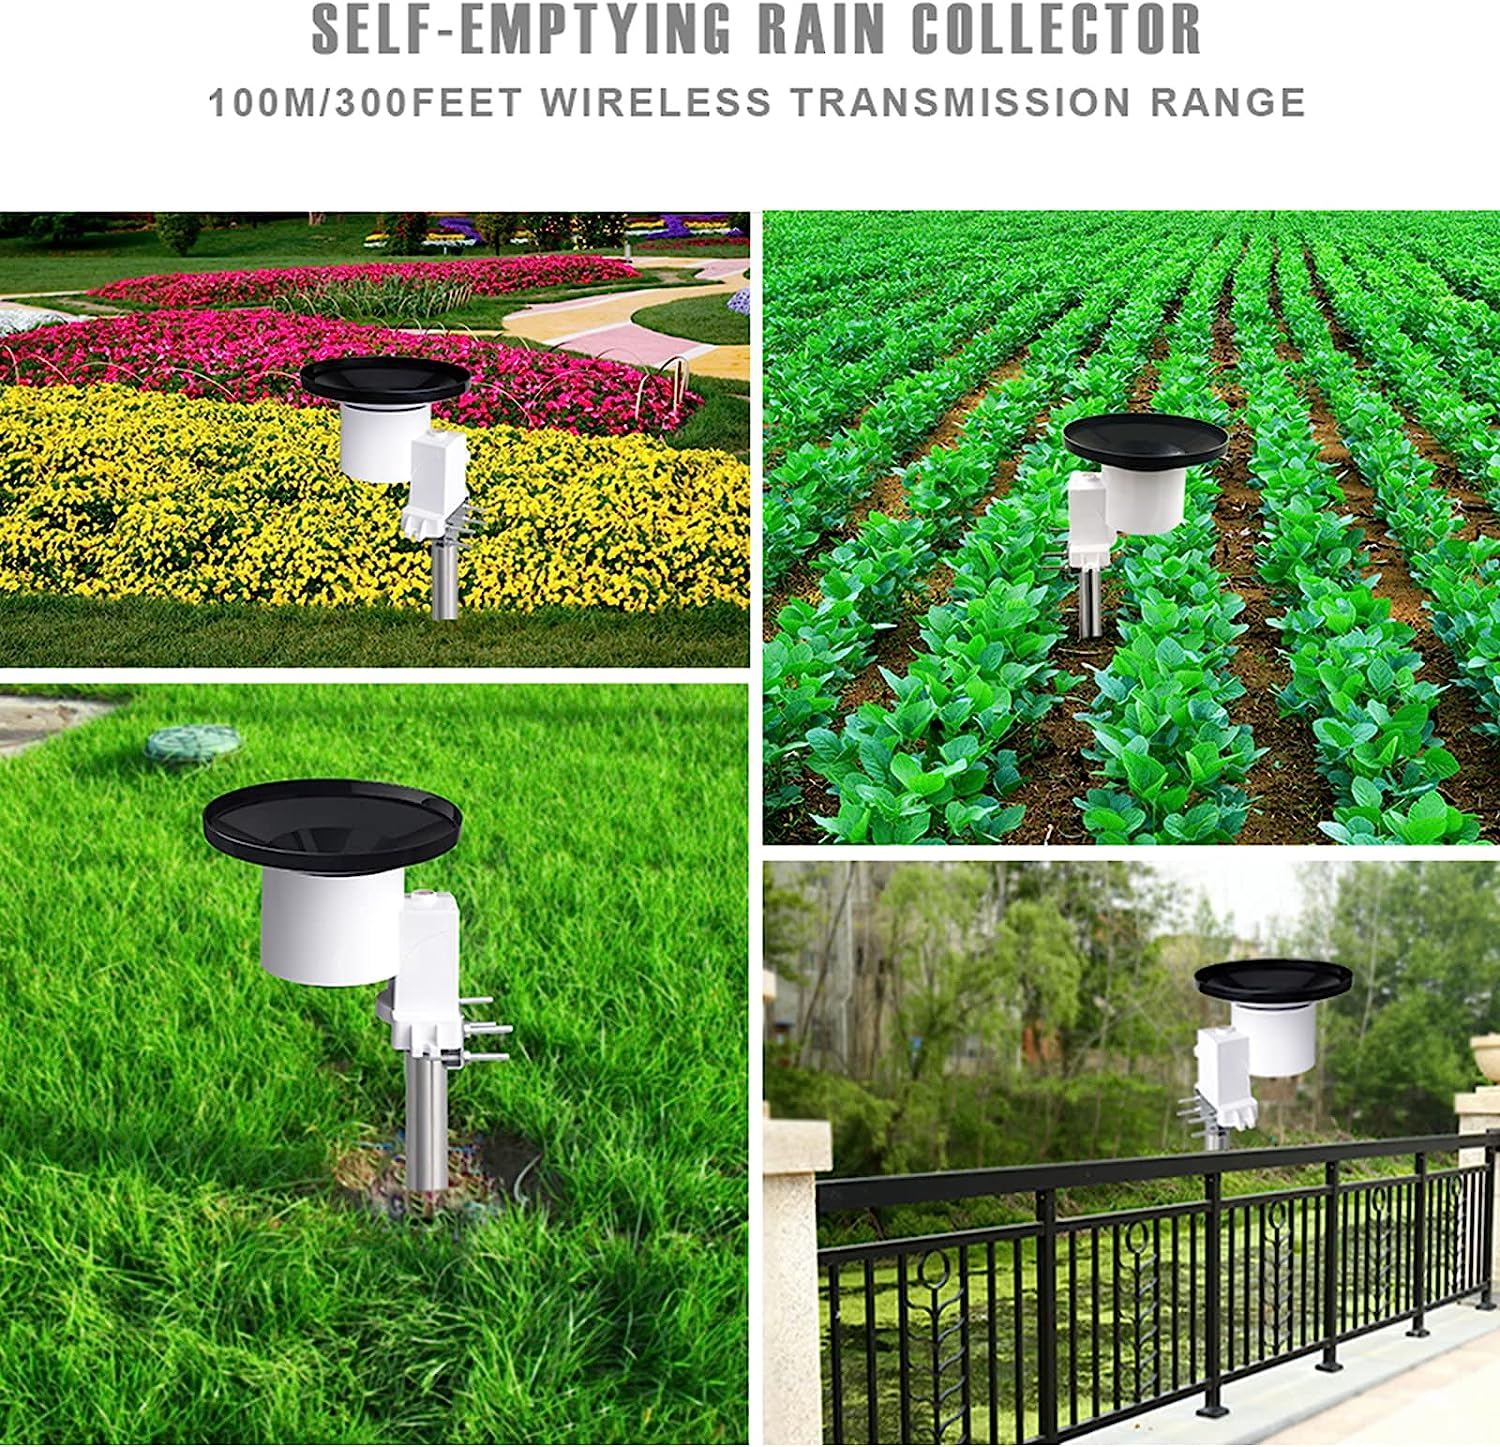
\includegraphics[scale=0.15]{rain-gaunt.jpg}
\end{frame}

\begin{frame}
  \frametitle{How to configure for AWS cloud?}
  \begin{itemize}
    \item Getting JSON data directly via ecowitt website ( Gateway)
      \begin{itemize}
        \item Configure the device to upload the data to ECowitt Server.
	\item Then, fetch the data or make an API call (lambda function) to produce the data for dynamoDB.
      \end{itemize}
    \item Send the sensors data to a mini server and convert it to mqtt. Refer source: \url{https://github.com/bachya/ecowitt2mqtt}{ecowitt-to-mqtt}
    \item Refer source: \url{https://www.cougar.eu.com/useful-guides/weewx-guides/rasberry-pi/add-ecowitt/index.html} {Raspberry Pi Guide}
  \end{itemize}

\end{frame}

\begin{frame}
  \frametitle{LORAWAN}
  \framesubtitle{Why?}
  \begin{itemize}
    \item  Arduino compabitle and Raspberry Pi Compatible
    \item  Radio Technology (LORAWAN vs Wifi).
    \item  LORA + WAN (cover up to 3 kilometers).
    \item  LoRA gateway (for soil moisture, rain sensor, and light sensors).
    \item  How to build one?
    \begin{itemize}
      \item Purchase the add-on hat for raspberry pi 4
      \item Convert it to LORAWAN internet gateway.
    \end{itemize}
  \end{itemize}

 \end{frame}

\begin{frame}
  \frametitle{LoRaWAN Gateway Module}
  \begin{center}
  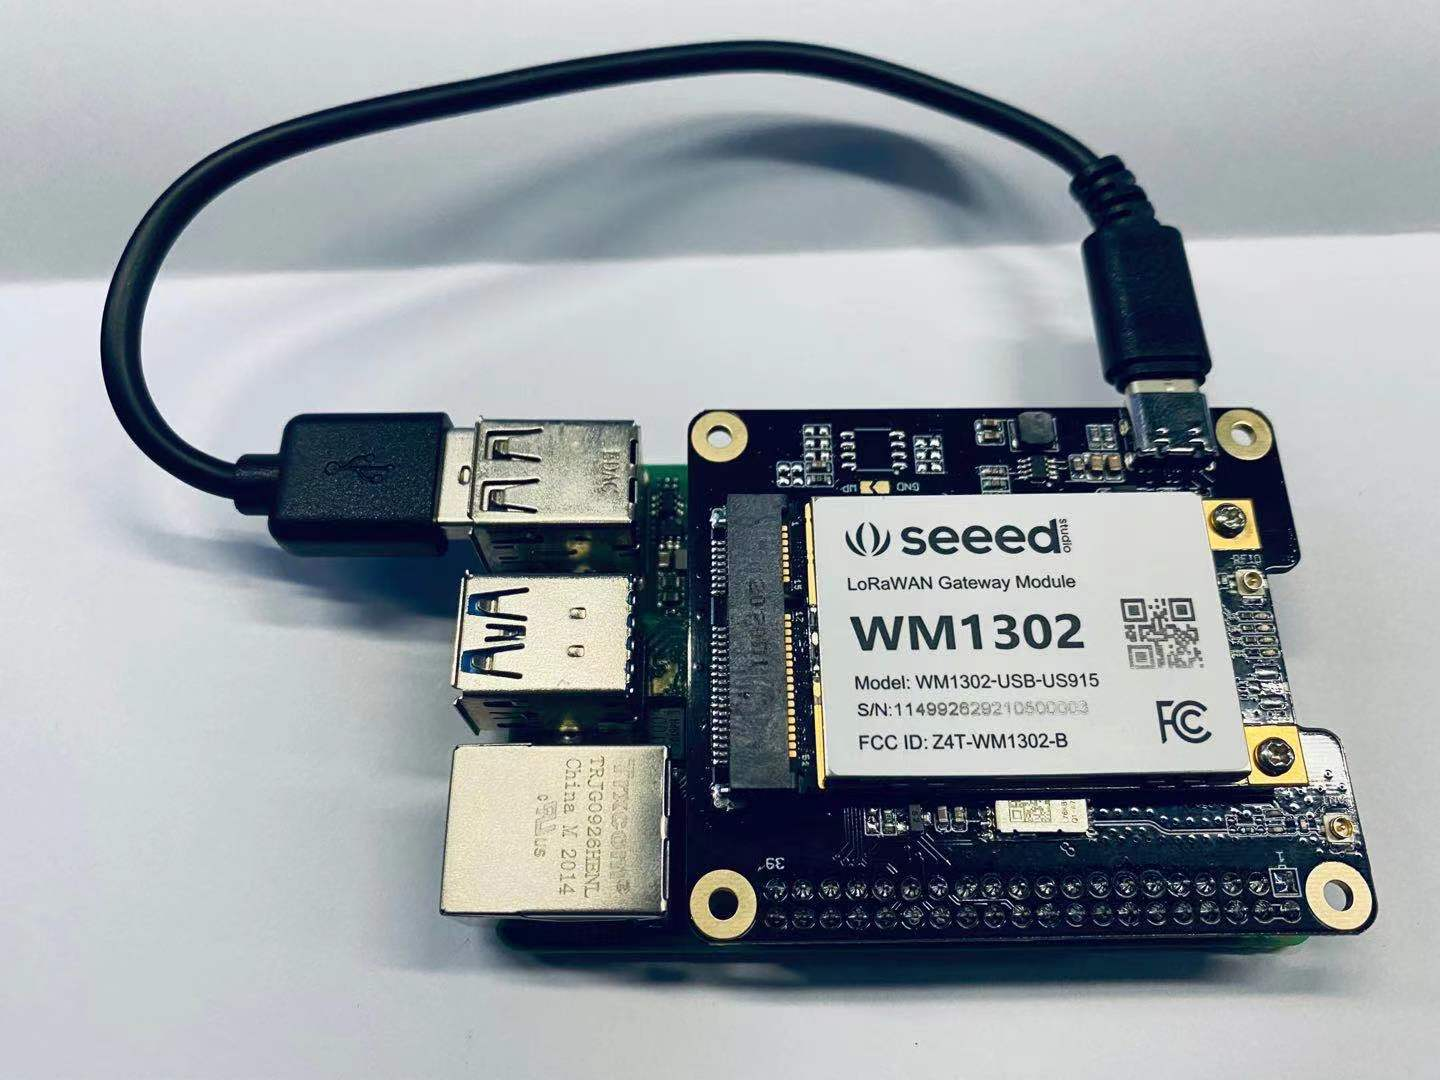
\includegraphics[scale=0.15]{lorawan-gateway.jpg}
  \end{center}

\end{frame}

\begin{frame}
  \frametitle{LoRaWAN Gateway Module}
  \begin{center}
  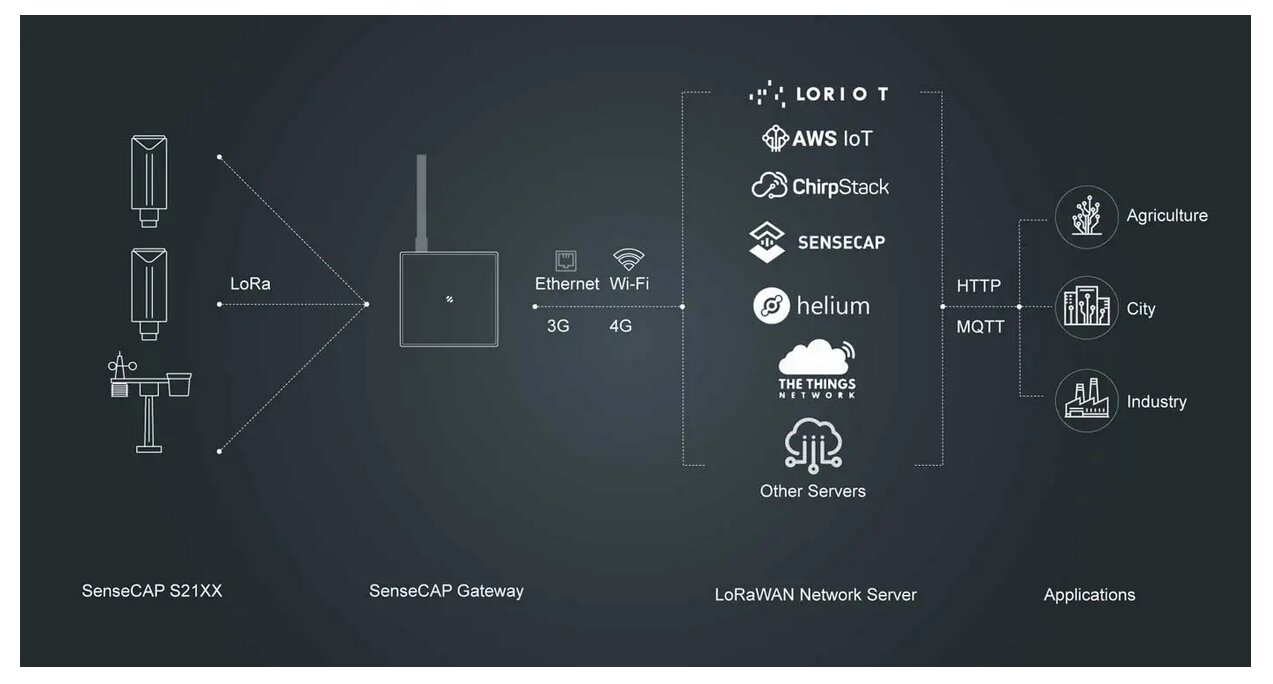
\includegraphics[scale=0.2]{lorawann-full-build.jpg}
  \end{center}
\end{frame}

\begin{frame}
  \frametitle{LoRaWAN Gateway Module}
  \framesubtitle{LoRaWAN Pump Control}
  \begin{center}
  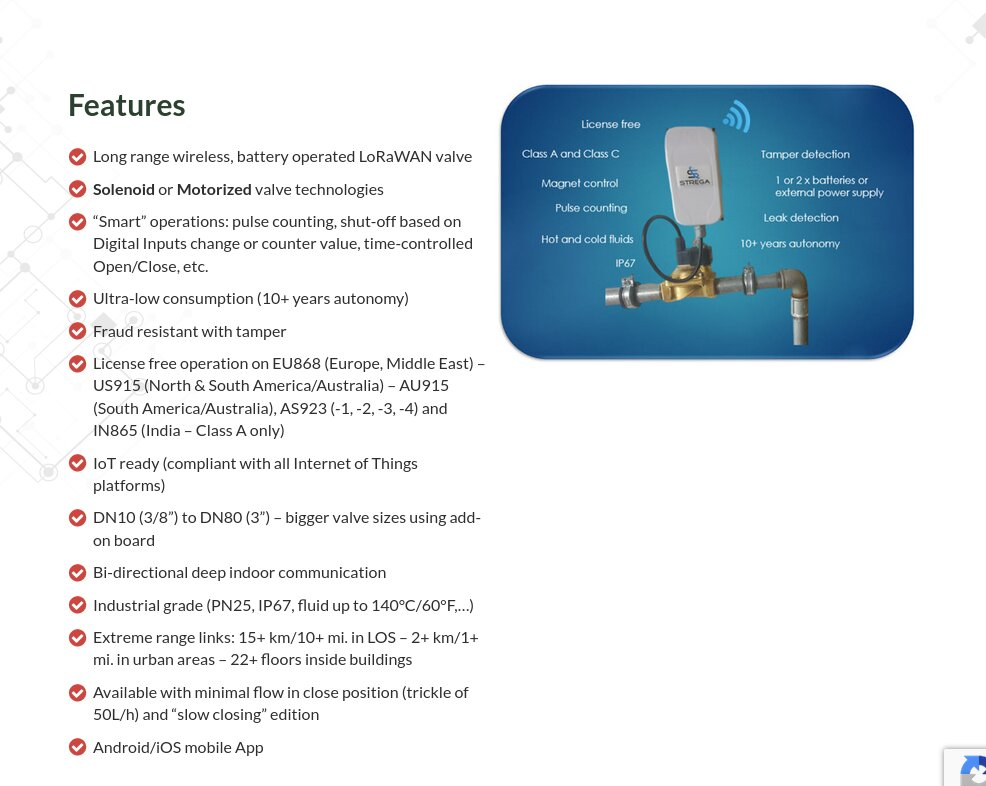
\includegraphics[scale=0.2]{solernoid-valve.jpg}
  \end{center}
\end{frame}


\begin{frame}[t]
  \frametitle{Help Needed}
 \begin{itemize}
   \item Install wifi for new sensor.
   \item Configure sensor for http request.
   \item Mount the equipment.
 \end{itemize} 
\end{frame}


\begin{frame}[t]
  \frametitle{Reference }
  \framesubtitle{Sources}
 \begin{itemize}
    \item \url{https://www.youtube.com/watch?v=ciL0MOtm50A&t=118s&ab_channel=MilesightIoT}{LORAWAN}
    \item \url{https://wiki.seeedstudio.com/WM1302_Pi_HAT/}{Pi HAT}
  \end{itemize}
  
  
\end{frame}


\end{document}
